\begin{abstract} \mdseries 
BrainGrid is an open-source neural-network simulator that is intended to aid scientists and researchers by providing prebuilt code that can be easily modified to fit different models. The program also offers the ability to easily transition to a GPU-centered with little additional work, and providing a potential speedup of up to a twentieth of the original runtime.

\begin{center}
	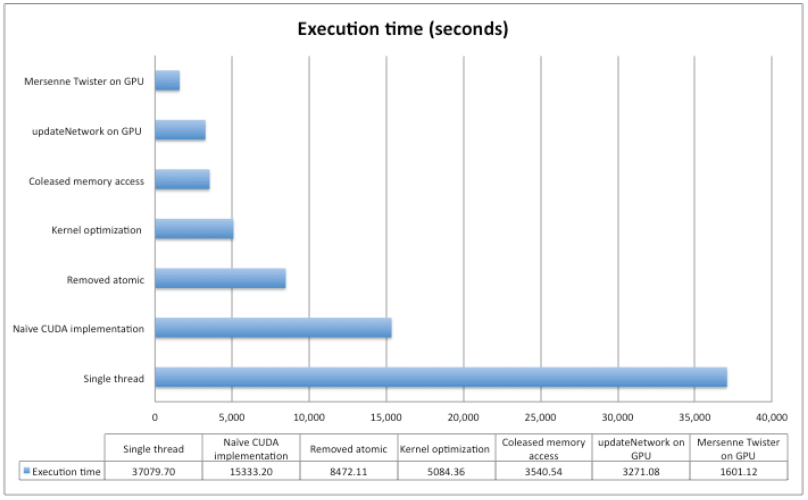
\includegraphics[width=\textwidth]{./images/SpeedComparison.PNG}
\end{center}

\noindent \mdseries The project began as an attempt to reduce the runtime of a simulation of a Leaky Integrate-and-Fire with more than a thousand neurons from two-thousand hours to a much more manageable runtime. Therefore, the program by default comes with a Leaky Integrate-and-Fire simulation preprogrammed. 
\end{abstract}
\pagebreak
